\chapter{Sortieralgorithmen (Klassifikation)}

\section*{Lösung}

\begin{itemize}
    \item Stabile Verfahren bewahren die Reihenfolge der Datensätze, falls deren Sortierschlüssel gleich sind.
    \item Bei internen Verfahren werden alle Datensätze im Hauptspeicher gehalten.
\end{itemize}


\section*{Anmerkungen und Ergänzungen}

Externe Verfahren sortieren Datensätze auf Externspeichern wie bspw. Magnetbänder (vgl.~\cite[141 ff.]{OW17b}). Hierfür müssen \textit{extern} zu sortierende Daten in Teilen in den Hauptspeicher geladen werden, im Gegensatz zu rein \textit{internen} Verfahren, die alle Datensätze im Hauptspeicher halten. \\

\textbf{in situ} bzw. \textbf{in place} Verfahren sortieren Schlüssel in einem Feld alleine durch Vertauschen \textit{innerhalb} des Feldes (vgl.~\cite[169]{GD18e}), ohne zusätzlich angelegte Felder zu nutzen.
Ein Beispiel für eine \textit{in situ}-Sortierung ist Bubble Sort, bei dem direkt benachbarte Elemente getauscht werden, wenn sie in der falschen Reihenfolge zueinander stehen.
Bei \textbf{Merge Sort} werden hingegen in Teilschritten Felder angelegt, die jeweils einen Ausschnitt der zu sortierenden Daten beinhalten (vgl.~\cite[112 ff.]{OW17b}). \\

Mit \textit{Merge Sort} als Beispiel kann auch die Aussage widerlegt werden, dass \textit{in place}-Verfahren nur genau den Hauptspeicher belegen, der von den zu sortierenden Elementen schon belegt ist: Wenn ein Feld der Länge $n$ gegeben ist, werden $2 * n - 2$ zusätzliche Felder in den Teilschritten angelegt - es wird also zusätzlicher Speicher angefordert.
\\

Per Defintion bewahren \textbf{stabile Verfahren} die relative Reihenfolge der Daten bei. Ein Beispiel für ein nicht-stabiles Verfahren ist \textbf{Selection Sort}.
Im folgenden werden die Schlüssel $1, 4_1, 5, 4_2, 2$ sortiert.
Da die $4$ mehrfach vorkommt, ist sie entsprechender der ursprünglichen Reihenfolge nummeriert.
Abbildung \ref{fig:unstablesort} stellt die Sortierung dar.
Im letzten Schritt haben $4_1$ und $4_2$ ihre Reigenfolge getauscht.



\begin{figure}[h]
    \centering
    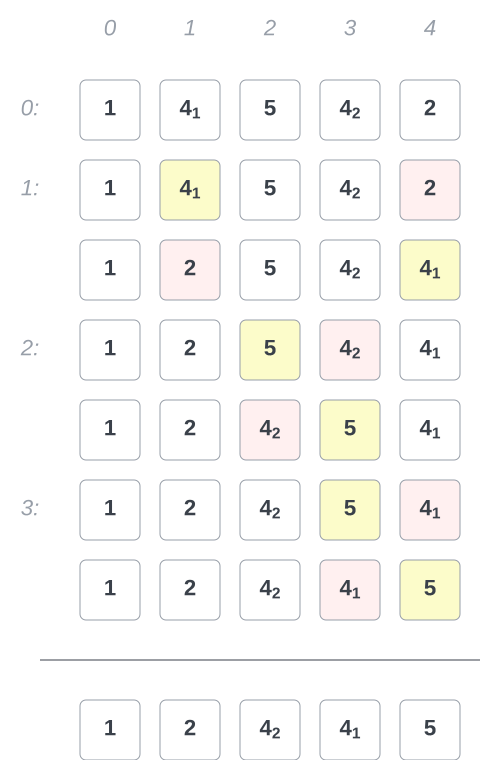
\includegraphics[
        width=8cm,
        keepaspectratio,
    ]{chapters/7. Sortieralgorithmen (Klassifikation)/img/unstablesort.png}
    \caption{Ein Beispiel für eine instabile Sortierung (Selection Sort): Nach Durchführung des Verfahrens ist die Reihenfolge von $4_1$ und $4_2$ vertauscht.}
    \label{fig:unstablesort}
\end{figure}

